%%%% For double-blind review submission, w/o CCS and ACM Reference (max submission space)
\documentclass[10pt, sigplan]{acmart}
%%\settopmatter{printfolios=true,printccs=false,printacmref=false}
%% For double-blind review submission, w/ CCS and ACM Reference
%\documentclass[sigplan,10pt,review,anonymous]{acmart}\settopmatter{printfolios=true}
%% For single-blind review submission, w/o CCS and ACM Reference (max submission space)
%\documentclass[sigplan,10pt,review]{acmart}\settopmatter{printfolios=true,printccs=false,printacmref=false}
%% For single-blind review submission, w/ CCS and ACM Reference
%\documentclass[sigplan,10pt,review]{acmart}\settopmatter{printfolios=true}
%% For final camera-ready submission, w/ required CCS and ACM Reference
%\documentclass[sigplan,10pt]{acmart}\settopmatter{}


%% Conference information
%% Supplied to authors by publisher for camera-ready submission;
%% use defaults for review submission.
%\acmConference[PL'17]{ACM SIGPLAN Conference on Programming Languages}{January 01--03, 2017}{New York, NY, USA}
%\acmYear{2017}
%\acmISBN{} % \acmISBN{978-x-xxxx-xxxx-x/YY/MM}
%\acmDOI{} % \acmDOI{10.1145/nnnnnnn.nnnnnnn}
%\startPage{1}

%% Copyright information
%% Supplied to authors (based on authors' rights management selection;
%% see authors.acm.org) by publisher for camera-ready submission;
%% use 'none' for review submission.
\setcopyright{none}
%\setcopyright{acmcopyright}
%\setcopyright{acmlicensed}
%\setcopyright{rightsretained}
%\copyrightyear{2017}           %% If different from \acmYear

%% Bibliography style

%\bibliographystyle{ACM-Reference-Format}

\citestyle{acmnumeric}   


%%%%%%%%%%%%%%%%%%%%%%%%%%%%%%%%%%%%%%%%%%%%%%%%%%%%%%%%%%%%%%%%%%%%%%
%% Note: Authors migrating a paper from traditional SIGPLAN
%% proceedings format to PACMPL format must update the
%% '\documentclass' and topmatter commands above; see
%% 'acmart-pacmpl-template.tex'.
%%%%%%%%%%%%%%%%%%%%%%%%%%%%%%%%%%%%%%%%%%%%%%%%%%%%%%%%%%%%%%%%%%%%%%


%% Some recommended packages.
\usepackage{booktabs}   %% For formal tables:
                        %% http://ctan.org/pkg/booktabs
\usepackage{subcaption} %% For complex figures with subfigures/subcaptions
                        %% http://ctan.org/pkg/subcaption
\usepackage{xspace}
\usepackage{graphicx}
\usepackage{ifthen}
\usepackage{pgfplots}
\usepackage{listings}
\usepackage{multirow}
\usepgfplotslibrary{statistics}
\usepackage{dblfloatfix} %enable fig at bottom of page
%



% Source Code
%\usepackage{color}
%\usepackage{textcomp}
%\usepackage{listings}
%\usepackage{ulem}
%\usepackage[T1]{fontenc}
%\usepackage{times}
% \usepackage{needspace}
 

% Source Code
\usepackage{color}
\usepackage{textcomp}
\usepackage{listings}

\definecolor{source}{gray}{0.85}% my comment style
\newcommand{\myCommentStyle}[1]{{\footnotesize\sffamily\color{gray!100!white} #1}}
%\newcommand{\myCommentStyle}[1]{{\footnotesize\sffamily\color{black!100!white} #1}}

% my string style
\newcommand{\myStringStyle}[1]{{\footnotesize\sffamily\color{violet!100!black} #1}}
%\newcommand{\myStringStyle}[1]{{\footnotesize\sffamily\color{black!100!black} #1}}

% my symbol style
\newcommand{\mySymbolStyle}[1]{{\footnotesize\sffamily\color{violet!100!black} #1}}
%\newcommand{\mySymbolStyle}[1]{{\footnotesize\sffamily\color{black!100!black} #1}}

% my keyword style
\newcommand{\myKeywordStyle}[1]{{\footnotesize\sffamily\color{green!70!black} #1}}
%\newcommand{\myKeywordStyle}[1]{{\footnotesize\sffamily\color{black!70!black} #1}}

% my global style
\newcommand{\myGlobalStyle}[1]{{\footnotesize\sffamily\color{blue!100!black} #1}}
%\newcommand{\myGlobalStyle}[1]{{\footnotesize\sffamily\color{black!100!black} #1}}

% my number style
\newcommand{\myNumberStyle}[1]{{\footnotesize\sffamily\color{brown!100!black} #1}}
%\newcommand{\myNumberStyle}[1]{{\footnotesize\sffamily\color{black!100!black} #1}}

\lstset{
language={},
% characters
tabsize=3,
escapechar={!},
keepspaces=true,
breaklines=true,
alsoletter={\#},
literate={\$}{{{\$}}}1,
breakautoindent=true,
columns=fullflexible,
showstringspaces=false,
% background
frame=single,
aboveskip=1em, % automatic space before
framerule=0pt,
basicstyle=\footnotesize\sffamily\color{black},
keywordstyle=\myKeywordStyle,% keyword style
commentstyle=\myCommentStyle,% comment style
frame=single,%
backgroundcolor=\color{source},
% numbering
stepnumber=1,
numbersep=10pt,
numberstyle=\tiny,
numberfirstline=true,
% caption
captionpos=b,
% formatting (html)
moredelim=[is][\bfseries]{<b>}{</b>},
moredelim=[is][\textit]{<i>}{</i>},
moredelim=[is][\underbar]{<u>}{</u>},
moredelim=[is][\color{red}\uwave]{<wave>}{</wave>},
moredelim=[is][\color{red}\sout]{<del>}{</del>},
moredelim=[is][\color{blue}\underbar]{<ins>}{</ins>},
% smalltalk stuff
morecomment=[s][\myCommentStyle]{"}{"},
%    morecomment=[s][\myvs]{|}{|},
morestring=[b][\myStringStyle]',
moredelim=[is][]{<sel>}{</sel>},
moredelim=[is][]{<rcv>}{</rcv>},
moredelim=[is][\itshape]{<symb>}{</symb>},
moredelim=[is][\scshape]{<class>}{</class>},
morekeywords={true,false,nil,self,super,thisContext},
identifierstyle=\idstyle,
}

\makeatletter
\newcommand*\idstyle[1]{%
\expandafter\id@style\the\lst@token{#1}\relax%
}
\def\id@style#1#2\relax{%
\ifnum\pdfstrcmp{#1}{\#}=0%
% this is a symbol
\mySymbolStyle{\the\lst@token}%
\else%
\edef\tempa{\uccode`#1}%
\edef\tempb{`#1}%
\ifnum\tempa=\tempb%
% this is a global
\myGlobalStyle{\the\lst@token}%
\else%
\the\lst@token%
\fi%
\fi%
}
\makeatother


%\newcommand{\ct}{\lstinline[backgroundcolor=\color{white}]}
%\newcommand{\needlines}[1]{\Needspace{#1\baselineskip}}
\newcommand{\lct}{\texttt}

\lstnewenvironment{code}{%
    \lstset{%
    % frame=lines,
    frame=single,
    framerule=0pt,
    mathescape=false
    }%
    \noindent%
    \minipage{\linewidth}%
}{%
    \endminipage%
}%


\lstnewenvironment{codeWithLineNumbers}{%
    \lstset{%
    % frame=lines,
    frame=single,
    framerule=0pt,
    mathescape=false,
    numbers=left
    }%
    \noindent%
    \minipage{\linewidth}%
}{%
    \endminipage%
}%



\newenvironment{codeNonSmalltalk}
{\begin{alltt}\sffamily}
{\end{alltt}\normalsize}



\usepackage{xcolor}
\newcommand{\todo}[1]{\color{orange}\fbox{\bfseries\sffamily\scriptsize TODO:}{\sf\small$\blacktriangleright$\textit{#1}$\blacktriangleleft$}\color{black}}
\newcommand{\sd}[1]{\color{red}\fbox{\bfseries\sffamily\scriptsize Stef:}{\sf\small$\blacktriangleright$\textit{#1}$\blacktriangleleft$}\color{black}}
\newcommand{\sk}[1]{\color{blue}\fbox{\bfseries\sffamily\scriptsize Sophie:}{\sf\small$\blacktriangleright$\textit{#1}$\blacktriangleleft$}\color{black}}
\newcommand{\cba}[1]{\color{purple}\fbox{\bfseries\sffamily\scriptsize Clement:}{\sf\small$\blacktriangleright$\textit{#1}$\blacktriangleleft$}\color{black}}
%\newcommand*{rotatebox{75}}




% Source Code
%\usepackage{color}
%\usepackage{textcomp}
%\usepackage{listings}
%\usepackage{ulem}
%\usepackage[T1]{fontenc}
%\usepackage{times}
% \usepackage{needspace}
 

% Source Code
\usepackage{color}
\usepackage{textcomp}
\usepackage{listings}

\definecolor{source}{gray}{0.85}% my comment style
\newcommand{\myCommentStyle}[1]{{\footnotesize\sffamily\color{gray!100!white} #1}}
%\newcommand{\myCommentStyle}[1]{{\footnotesize\sffamily\color{black!100!white} #1}}

% my string style
\newcommand{\myStringStyle}[1]{{\footnotesize\sffamily\color{violet!100!black} #1}}
%\newcommand{\myStringStyle}[1]{{\footnotesize\sffamily\color{black!100!black} #1}}

% my symbol style
\newcommand{\mySymbolStyle}[1]{{\footnotesize\sffamily\color{violet!100!black} #1}}
%\newcommand{\mySymbolStyle}[1]{{\footnotesize\sffamily\color{black!100!black} #1}}

% my keyword style
\newcommand{\myKeywordStyle}[1]{{\footnotesize\sffamily\color{green!70!black} #1}}
%\newcommand{\myKeywordStyle}[1]{{\footnotesize\sffamily\color{black!70!black} #1}}

% my global style
\newcommand{\myGlobalStyle}[1]{{\footnotesize\sffamily\color{blue!100!black} #1}}
%\newcommand{\myGlobalStyle}[1]{{\footnotesize\sffamily\color{black!100!black} #1}}

% my number style
\newcommand{\myNumberStyle}[1]{{\footnotesize\sffamily\color{brown!100!black} #1}}
%\newcommand{\myNumberStyle}[1]{{\footnotesize\sffamily\color{black!100!black} #1}}

\lstset{
language={},
% characters
tabsize=3,
escapechar={!},
keepspaces=true,
breaklines=true,
alsoletter={\#},
literate={\$}{{{\$}}}1,
breakautoindent=true,
columns=fullflexible,
showstringspaces=false,
% background
frame=single,
aboveskip=1em, % automatic space before
framerule=0pt,
basicstyle=\footnotesize\sffamily\color{black},
keywordstyle=\myKeywordStyle,% keyword style
commentstyle=\myCommentStyle,% comment style
frame=single,%
backgroundcolor=\color{source},
% numbering
stepnumber=1,
numbersep=10pt,
numberstyle=\tiny,
numberfirstline=true,
% caption
captionpos=b,
% formatting (html)
moredelim=[is][\bfseries]{<b>}{</b>},
moredelim=[is][\textit]{<i>}{</i>},
moredelim=[is][\underbar]{<u>}{</u>},
moredelim=[is][\color{red}\uwave]{<wave>}{</wave>},
moredelim=[is][\color{red}\sout]{<del>}{</del>},
moredelim=[is][\color{blue}\underbar]{<ins>}{</ins>},
% smalltalk stuff
morecomment=[s][\myCommentStyle]{"}{"},
%    morecomment=[s][\myvs]{|}{|},
morestring=[b][\myStringStyle]',
moredelim=[is][]{<sel>}{</sel>},
moredelim=[is][]{<rcv>}{</rcv>},
moredelim=[is][\itshape]{<symb>}{</symb>},
moredelim=[is][\scshape]{<class>}{</class>},
morekeywords={true,false,nil,self,super,thisContext},
identifierstyle=\idstyle,
}

\makeatletter
\newcommand*\idstyle[1]{%
\expandafter\id@style\the\lst@token{#1}\relax%
}
\def\id@style#1#2\relax{%
\ifnum\pdfstrcmp{#1}{\#}=0%
% this is a symbol
\mySymbolStyle{\the\lst@token}%
\else%
\edef\tempa{\uccode`#1}%
\edef\tempb{`#1}%
\ifnum\tempa=\tempb%
% this is a global
\myGlobalStyle{\the\lst@token}%
\else%
\the\lst@token%
\fi%
\fi%
}
\makeatother


%\newcommand{\ct}{\lstinline[backgroundcolor=\color{white}]}
%\newcommand{\needlines}[1]{\Needspace{#1\baselineskip}}
\newcommand{\lct}{\texttt}

\lstnewenvironment{code}{%
    \lstset{%
    % frame=lines,
    frame=single,
    framerule=0pt,
    mathescape=false
    }%
    \noindent%
    \minipage{\linewidth}%
}{%
    \endminipage%
}%


\lstnewenvironment{codeWithLineNumbers}{%
    \lstset{%
    % frame=lines,
    frame=single,
    framerule=0pt,
    mathescape=false,
    numbers=left
    }%
    \noindent%
    \minipage{\linewidth}%
}{%
    \endminipage%
}%



\newenvironment{codeNonSmalltalk}
{\begin{alltt}\sffamily}
{\end{alltt}\normalsize}



\begin{document}

%%%
% Keyword definition (so I can change it once for all)
%%%

\def\openSmalltalkVM{Open-Smalltalk-VM\xspace}
%%%
% End Legend
%%%

%% Title information
\title[Over Twenty Years of Virtual Machine Development Through Simulation]{Over Twenty Years of Virtual Machine Development and Debugging Through Simulation}

%% Author with single affiliation.
\author{Eliot Miranda}
                                        %% can be repeated if necessary
\affiliation{
  %\position{Position1}
 % \department{VM team}              %% \department is recommended
  \institution{Feenk}            %% \institution is required
 % \streetaddress{Street1 Address1}
  \city{San Francisco}
  %\state{France}
  %\postcode{Post-Code1}
  \country{California}                    %% \country is recommended
}
\email{eliot.miranda@gmail.com}          %% \email is recommended

%% Author with two affiliations and emails.
\author{Cl\'ement B\'era}
\affiliation{
  % \position{}
	\department{Software Languages Lab}              %% \department is recommended
	\institution{Vrije Universiteit Brussel}            %% \institution is required
	\city{Brussel}
  % \state{}
  % \postcode{}
	\country{Belgium}                    %% \country is recommended
}
\email{clement.bera@vub.ac.be}          %% \email is recommended

%% Author with two affiliations and emails.
\author{Elisa Gonzalez Boix}
\affiliation{
  % \position{}
	\department{Software Languages Lab}              %% \department is recommended
	\institution{Vrije Universiteit Brussel}            %% \institution is required
	\city{Brussel}
  % \state{}
  % \postcode{}
	\country{Belgium}                    %% \country is recommended
}
\email{egonzale@vub.ac.be}          %% \email is recommended


%% Abstract
%% Note: \begin{abstract}...\end{abstract} environment must come
%% before \maketitle command
\begin{abstract}

\openSmalltalkVM was originally written in Smalltalk to specify and example the virtual machine (VM) implementation. The same code base was changed a little bit to allow Smalltalk-to-C compilation to generate the production VM through the C compiler. Two execution models are effectively available, simulation, where the Smalltalk code is executed on top of a Smalltalk VM, and production, where the same code is compiled to executable code through the C compiler. Simulation is used to develop and debug the VM. Production is used to release the VM. 

As the VM evolved, by introducing better garbage collector algorithms or a just-in-time compiler, both execution models co-evolved. For example, the simulation infrastructure was extended with a processor simulator to simulate the code generated by the just-in-time compiler. 

In this paper, we detail the VM simulation infrastructure and we report our experience developing and debugging the VM within it. We mention some of the limitations and how we worked around them. We discuss specifically how we use the VM simulator to develop and debug two core VM components, the garbage collector and the just-in-time compiler. Then, we discuss how we use the simulation infrastructure to perform analysis on the runtime, directing some design decisions we make to tune the VM performance.

\end{abstract}

%% 2012 ACM Computing Classification System (CSS) concepts
%% Generate at 'http://dl.acm.org/ccs/ccs.cfm'.
%\begin{CCSXML}
%<ccs2012>
%<concept>
%<concept_id>10011007.10011006.10011008</concept_id>
%<concept_desc>Software and its engineering~General programming languages</concept_desc>
%<concept_significance>500</concept_significance>
%</concept>
%<concept>
%<concept_id>10003456.10003457.10003521.10003525</concept_id>
%<concept_desc>Social and professional topics~History of programming languages</concept_desc>
%<concept_significance>300</concept_significance>
%</concept>
%</ccs2012>
%\end{CCSXML}

%\ccsdesc[500]{Software and its engineering~General programming languages}
%\ccsdesc[300]{Social and professional topics~History of programming languages}
%% End of generated code


%% Keywords
%% comma separated list
\keywords{Just-in-Time compiler, Virtual machine, Managed runtime, Tools}  %% \keywords are mandatory in final camera-ready submission


%% \maketitle
%% Note: \maketitle command must come after title commands, author
%% commands, abstract environment, Computing Classification System
%% environment and commands, and keywords command.
\maketitle

\section{Introduction}
\label{sec:intro}

To specify the language and explain how to write the virtual machine (VM) for it, the Smalltalk-80 crew wrote a Smalltalk VM entirely in Smalltalk \cite{blueBook}. In 1995, the same team built an open-source Smalltalk and VM, Squeak \cite{SqueakByExample}. The VM was ported from the original specifications. Part of the code base was however narrowed down to a subset of Smalltalk, called \emph{Slang}, to allow Smalltalk to C compilation \cite{BackToTheFuture} and generate an efficient VM through the C compiler. Effectively, the VM could be both simulated by executing the Slang code on top of the Smalltalk VM or compiled through the C compiler to native code to generate the production VM. At this point, the VM consisted mainly in:
\begin{itemize}
\item an interpreter with a spaghetti stack, 
\item a memory manager with a generational garbage collector (GC) and
\item BitBlt, an extension for the user interface bit-based engine.
\end{itemize} 
These three parts of the VM were written entirely in Slang. A few extra features, such as file management, were written both in Smalltalk for simulation purposes and in C for the production VM.

Over the years, the Squeak VM evolved to give birth recently to \openSmalltalkVM\footnote{https://github.com/OpenSmalltalk/opensmalltalk-vm/}, the default VM for different Smalltalk and Smalltalk-like runtimes such as Pharo \cite{PharoByExample}, Squeak \cite{SqueakByExample}, Cuis, Croquet and NewSpeak \cite{NewspeakOopsla}. As the VM evolved, the simulator co-evolved as a tool to develop and debug the VM. The most significant evolution of the simulator came with the introduction of the Just-In-Time compiler (JIT). The existing simulator was not able to simulate the machine code generated by the JIT and had to be extended by binding multiple processor simulators (Bochs for x86 \& x64, SkyEye for ARMv6).

In the following section, we explain the VM infrastructure with both the compilation pipeline to generate the production VM and the simulation infrastructure used to develop and debug the VM. Section \ref{sec:GCExp} and Section \ref{sec:JITExp}  reports our experience developing respectively the full GC and the JIT with our infrastructure. Section \ref{sec:Analysis} shows how we abuse the simulator to analyse the runtime and direct design decisions to improve performance. Lastly, we discuss some related work and conclude.

\section{Virtual Machine Infrastructure}
\label{sec:VMSimulation}

As shown in Figure \ref{fig:VMCompilation}, the VM code base is written both in Slang and in C. The Core VM code (the interpreter, the JIT and the memory manager), is written in Slang. The platform code, \emph{i.e.,} Operating System dependent code such as file management or I/O is written directly in C. 
%EXPLAIN scientifically in this part - no history. + FIGURE, basic with design. 

\begin{figure}[bth!]
		\centering
		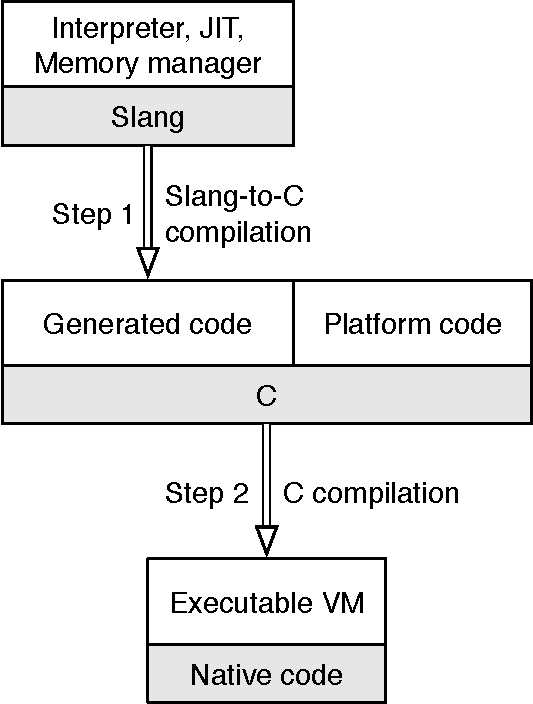
\includegraphics[width=0.55\linewidth]{figures/VMCompilation}
		\caption{Cog VM compilation}
		\label{fig:VMCompilation}
\end{figure}

The VM executable is generated in a two step process. Firstly, the Slang-to-C compiler translates the Slang code to C code, generating a few files. This first step takes several seconds. Secondly, the C compiler (depending on the platform, LLVM or GCC), translates the C code into an executable. This second step may take several dozens of seconds the first time, then, depending on what the programmer changed and what the C compiler have cached, it usually only takes a few seconds to recompile the C code. 

The VM can be compiled in two main flavours, interpreter-only or interpreter+JIT. Although the version with the JIT is used in production, the interpreter version is convenient for special purposes. For example, debugging the garbage collector or evaluating new language features without dealing can be done in the interpreter-only VM, avoiding the JIT complexity.

There are multiple reasons why we keep writing the core components in Slang and not in C/C++. Most of them are small details. For instance, the Slang-to-C compiler generates C code slightly different from the Slang code using different annotations. It can for example duplicate the implementation of specific methods with specific constant operands to generate more efficient code in the interpreter. The main reason why we keep using Slang over C/C++ is VM simulation. By interpreting the Slang code as Smalltalk code, emulating native code using an external processor simulator and simulating the memory using a large byte array, we are able to simulate the whole VM execution, allowing to develop and debug it with the Smalltalk development tools and a live programming experience.

\subsection{Simulating the Virtual Machine}

In this section, we firstly describe briefly the start-up sequence of \openSmalltalkVM using snapshots, a key aspect of the VM simulator success. Then, we detail the simulation of the interpreter-only VM. The simulation of the full VM is a superset and is explained in the last subsection.

\paragraph{Start-up from snapshots.} 
Smalltalk is a snapshot-based language. A Smalltalk program is started from a snapshot, \emph{i.e.,} a memory dump of all live objects at a given point in the execution of a program. The snapshot includes objects such as the classes, the compiled methods in the form of bytecodes and the running processes. At start-up, the VM restores the state of all objects in memory and resumes execution in the process active at snapshot time. 

When programming with Smalltalk, the programmers usually starts from a snapshot which contains the core libraries, the development environment and the application developed. Development of the application consists essentially in writing and editing code, which effectively installs, modifies and removes compiled methods and classes from the set of live objects. When the changes are done, the developer takes a new snapshot, which includes its changes. Deployment is performed using a snapshot containing the deployed application and the required core librairies (unused librairies and development tools may be removed from the deployed snapshot to decrease memory footprint and for security purposes).

Starting up \openSmalltalkVM from source files has never been possible. However, recent work~\cite{PharoBootstrap} allowed one of the Smalltalk runtime to recreate a snapshot from sources, indirectly allowing to start the VM from source files.

\paragraph{Interpreter-only simulation.} 
As the VM can be compiled with and without the JIT, the VM can also be simulated with or without the JIT. 

\begin{figure*}[ht!]
		\centering
		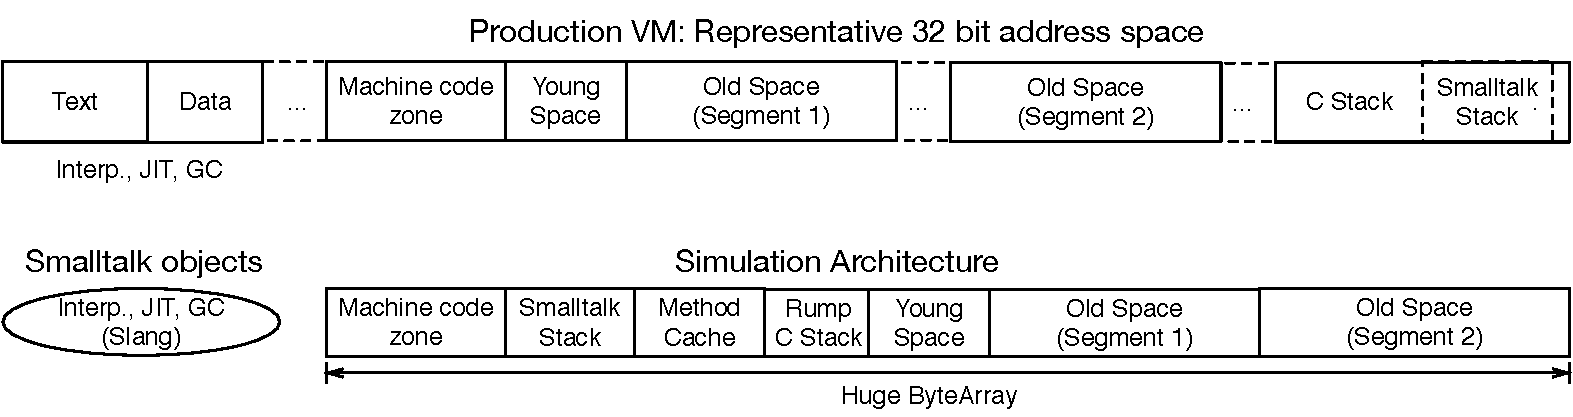
\includegraphics[width=0.9\linewidth]{figures/SimulatedMemory}
		\caption{Runtime Memory and Simulated Counter-Part}
		\label{fig:SimulatedMemory}
\end{figure*}

Figure \ref{fig:SimulatedMemory} describes, from a high-level perspective, the memory used by \openSmalltalkVM at runtime and the simulated counter-part. Let's detail briefly the memory used by the production VM, on the top of the figure. On the left side, which is usually the low addresses, we can find Text, the memory section holding the native code of the VM (the interpreter, the memory manager and the JIT itself, but not the code compiled by the JIT). Then, Data holds initialized and uninitialized data, mainly the C variables used globally in the VM. On higher addresses, we can find the beginning of the memory managed by the VM. At start-up, the VM mmaps a memory region used for the executable code generated by the JIT (optional executable section, exists only if the JIT is enabled), for the young objects and for the old objects present in the snapshot started plus a little more space for the first tenures\footnote{A tenure is the process of promoting young objects to old objects in a generational GC.} to be performed without triggering the full garbage collector. Later during execution, as old space grows, new memory regions are mmap'ed on higher addresses to store other old objects. Usually at very high addresses, we can find the C stack. Room in the C stack is alloca'ed at VM start-up to hold the Smalltalk stack. Both stacks are disjointed and managed differently. 

In the simulator, the heap is simulated as a large contiguous byte array. References between objects are effectively indexes inside the byte array instead of pointers. All the Slang variables, normally translated to C variabled, are simulated as Smalltalk objects. They used specific classes, such as \emph{CArrayAccessor} over normal Smalltalk classes, to emulate the C behavior (only array accesses are available in C, not high level iterator APIs, etc.). The Slang code is executed as Smalltalk code. The Smalltalk stack is represented in \openSmalltalkVM as a double linked list of stack pages which are maintained by the VM. Each stack page is represented as a Smalltalk object in the simulator.

All the Slang code is implemented in multiple Smalltalk classes, to organise the code and to add flexibility through polymorphism. For example, the AbstractCompactor class has two subclasses, one implements a sweep algorithm and the other a compact one. For production, at Slang-to-C compilation time, all the code is compiled in a single C file. All the flexibility is removed, using the same example, the VM developer chooses at this moment if he wants to compile a VM with a sweep or compact algorithm. No polymorphism is available at runtime. However, since polymorphism is available in the simulator, it can be abused for debugging purposes. Still re-using the same example, the AbstractCompactor class has also simulation specific subclasses. Such versions typically express additional constraints in the form of assertions which can be written in plain Smalltalk without restrictions to easily express complex constraints. They also keep specific values live so they can be accessed at debugging time.

In Simulation, one of the core feature is to be able to re-use the whole Smalltalk IDE, including the browser, the inspectors and the debugger to develop and debug the VM. Most new features can be develop and debug interactively, adding code to the VM at runtime, in the simulation environment, as for normal Smalltalk programs.

\paragraph{JIT simulation.} 

In addition to the interpreter simulator, simulating the JIT requires to simulate the execution of native code it generates. The JIT itself is written in Slang and simulated with the Smalltalk execution model. To simulate the machine code, the start of the byte array representing the memory holds, when the JIT is enabled, the machine code generated at runtime. 

Bindings to processor simulator libraries (Bochs for x86 and x64, Skyeye for ARMv6) were implemented so that the machine code can be simulated. Calls in-between slang code and direct machine code are a little bit trickier to simulate. Calls from machine code to slang code are implemented by using multiple invalid processor instructions, leading to a trap in the processor simulator. Such traps can be caught is the VM simulator, which then resumes Slang simulation by calling the correct method based on the invalid processor instruction. Calling machine code from Slang requires to start the machine code simulation but also to raise an exception to stop Slang simulation. Indeed, in the production VM, the processor can execute the C code or the native code generated by the JIT, but not both at the same time. 

Machine code simulation can be performed in two different ways. The processor simulator can start simulating code until it meets an invalid instruction. That version is convenient because it is the fastest to execute, while still catching errors such as invalid memory accesses. Alternatively, it can simulate one instruction at a time. This second version is slower, but it allows to implement specific debugging features, such as conditional breakpoints in-between each machine instruction.

\subsection{In-image compilation}

Simulating the whole VM requires going through the whole start-up sequence: loading the snapshot, running code registered in the start-up sequence and resuming the user interface. The whole start-up takes around 15 seconds on a recent Macbook pro. While developing the JIT, this start-up time may still be too long and move the live programming experience to an edit-compile-run cycle, which we want to avoid. 

To work around this problem, we implemented a tool called \emph{In-image compilation}. In-image compilation basically allows to call the JIT as a Smalltalk library on a given bytecode compiled method to generate the corresponding machine code, calls the bound processor simulator to disassemble the code and decorate the disassembly with Smalltalk specific information. To generate the machine code, the JIT has to access specific objects (the compiled method, the literals, known objects such as true, false or nil) as if they were in the simulated memory. To work around this, we built a facade, which includes mock addresses for all the object the JIT may require to generate the machine code of a given method. Figure \ref{fig:InImageCompiler} summarizes the process. Note that this technique applies for the baseline JIT, which translate a single bytecode method into machine code, adaptive optimizations and speculative optimizations are debugged differently.

\begin{figure}[ht!]
		\centering
		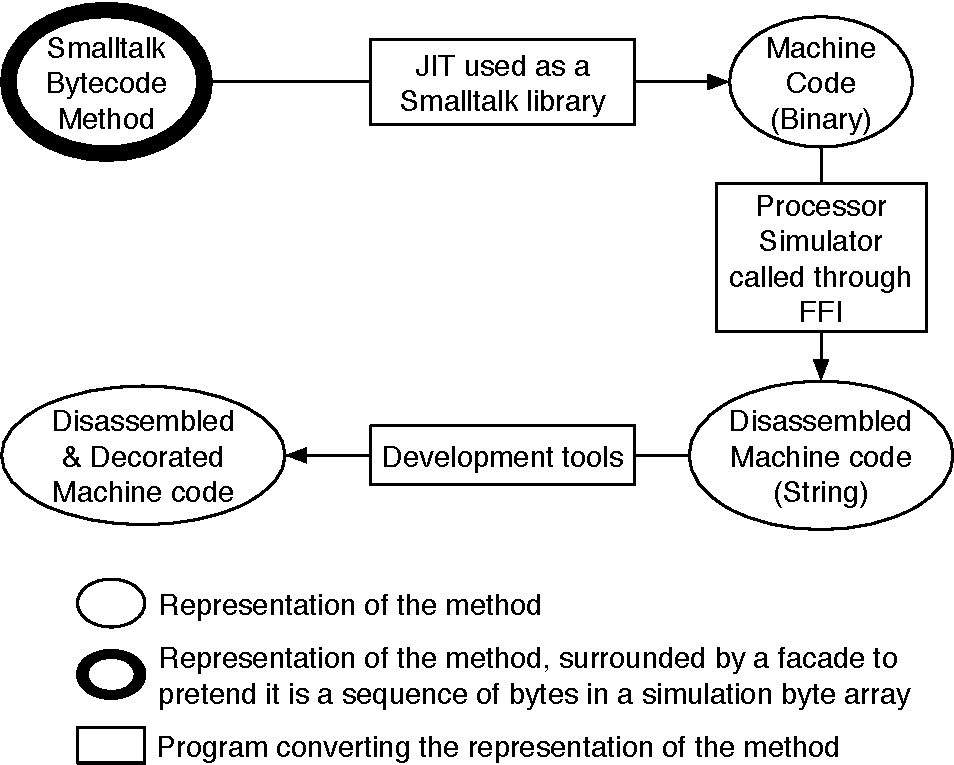
\includegraphics[width=\linewidth]{figures/InImageCompiler}
		\caption{In-image compilation}
		\label{fig:InImageCompiler}
\end{figure}

\paragraph{Templates.} The JIT generates a sequence of machine instructions for a given pattern of bytecodes. We will use the term template to describe the sequence of machine instructions generated for a pattern of bytecodes, even though we do not like to reduce the JIT to a simple template-based JIT since each bytecode generates slightly different machine instructions based on register pressure, a simulated stack and  
a few heuristics. Since the JIT is template-based, in-image compilation is very convenient to develop and optimize each of the JIT templates. 

\subsection{Virtual Machine Simulation Limitations}

The simulator has several limitations. Due to the simulation infrastructure being different from the actual hardware, code is run differently and one could think it leads to strange bugs happening only in simulation or in production. However, we have been using this infrastructure since 1995, and this kind of bugs are really rare and usually easy to fix. We have however two main limitations: simulation performance which is quite slow and calls to external C/C++/machine code which cannot be simulated.

\paragraph{Performance.}
The first limitation is due to the simulation performance. The interpreter-only is simulator is around 200 times slower to execute code than the normal VM. With the JIT and processor simulation enabled, without specific debugging options such as conditional breakpoints in between machine instructions, simulation drops to around 500 times slower than the normal VM. We usually enabled conditional breakpoints in-between machine instructions only when we reach a point in the simulator where the bug is about to happen since it is way slower, so the overall performance in this context is not really relevant.

This means for example that if a GC bug happens in an application 15 minutes after start-up, it will take 50 hours to reproduce in the interpreter-only simulator. Bugs in the jitted code are worse. Fortunately, we work around this problem by using snapshots and the interpreter-only simulator for GC bugs. In general, once we are able to reproduce a bug in the production VM, we try to snapshot the runtime just before it crashes. The VM simulator can then be started just before the crash and the debugging tools can be used after only several dozens of seconds. If the bug is unrelated to the JIT, the interpreter-only simulator can also be used and it is a little bit quicker to execute code.

\paragraph{Calls to external code.}
Although most of the GC and JIT development and debugging can be done in the simulator, specific tasks cannot be done this way. Basically, any calls outside of the machine code generated by the JIT and the Slang code cannot be simulated. For specific small parts of the VM, such as file management, we extended the simulator, effectively duplicating the code base with the C code, to support those features in simulation. However, there is no solution in the general case: we cannot afford to simulate both the compiled C code and the jitted code on the processor simulator, that would be horribly slow, and specific behaviors in the machine code not present in the code generated by the JIT can hardly be simulated (Access to C variables, OS variables, etc.).

The main limitation we have right now is with Foreign Function Interfaces (FFI). We have a significant amount of bugs in FFI, often due to specific interaction between call-backs, low-level assembly FFI specific glue code and moving objects. Such bugs cannot be debugged with our simulation infrastructure so far and we have to rely on gdb/lldb.

\section{Garbage Collection Development}
\label{sec:GCExp}

Recently, to evaluate new old space garbage collection algorithms we designed against standard algorithms, we implemented a Mark-Sweep in addition to the existing Mark-Compact collector. The whole implementation was done in the simulator, and only when it was working there, was it compiled to C. Using this process, the compiled C code was kind of working out of the box. To describe the implementation process, we need to discuss briefly first the assertion levels in the VM. Then we will show how we debugged the algorithm.

\paragraph{Assertions.}To stabilise our code base and find easily production bugs, all the code based is annotated with assertions. Each assertion ensures a specific state is as the VM developer would expect it to be and stops or log the incorrect result if not. We have a multi-level assertion system. Assertions written in plain Smalltalk are convenient since more complex constraints can be expressed easily using high level structures (Sets, etc.), but they can be performed only in the simulator. Assertions written in Slang are executed in the simulator but they are also compiled to C. The C compiler, based on a compilation flag, chooses to compile the VM with or without assertions. The VM with assertions is used for debugging and to recreate snapshots just before a VM crash. The VM without assertions is the production VM.

\paragraph{Simulation.} Once we had partially written the new Sweep algorithm, we started the simulator. Since the algorithm was partially written, we had to write the missing pieces inside the debugger, installing the new code at runtime, as one can do it in any Smalltalk application. In addition, the simulator has an interesting property: each time it performs a GC, either a scavenge or an old space collection, it first copies the simulated memory (\emph{i.e.,} the heap), performs the GC there, and if no assertion fails, it then performs the GC on the original version. This means that if the algorithm was not working, and likely an assertion would fail or an error such as incorrect memory access would be raised, the erratic behavior would have happened in a copy of the heap. The simulator can then reproduce the exact same erratic behavior as many times as the VM developer wants duplicating again and again the same original heap. This is very convenient to debug specific GC bugs. Indeed, often in GC bugs, when the bug happens, the memory is already corrupted and it's quite difficult to track back where the bug comes from without rewinding the memory state, which is usually very difficult or impossible.

\section{Just-in-Time Compiler Development}
\label{sec:JITExp}

We firstly discuss how we use the simulator to debug crashes in deployed applications, then how we use in-image compilation to develop the JIT itself.

\subsection{Debugging crashes with conditional breakpoints in machine code}

In the recent years, we added support for a more aggressive JIT with speculative optimizations through a bytecode to bytecode optimizer \cite{SistaFastStartUp}, re-using the existing template JIT as a back-end. To be able to generate efficient bytecodes in the bytecode to bytecode optimizer, we had to introduce new unsafe bytecodes allowing, for example, accesses in arrays without any checks (type and bounds checks) \cite{SistaBytecodeSet}. For each new bytecode, we introduced new templates in the existing JIT to generate efficient machine code for the optimized methods using the new bytecodes. Once all the basic unit tests worked, we ran the VM with the speculative optimizer, which executed optimized code, and got a crash. We could figure out which bytecode method was triggering the crash, but we had no idea from which template the crash came from. In addition, optimized methods include many inlined methods, making them very large, so it was difficult to figure out where the issue comes from just by looking at thousands of bytecodes.

To understand the crash, we created a snapshot where the faulty method was executed right after start-up. We started the VM simulator, and set-up a conditional breakpoint so that simulator would stop when the JIT would generate that method to machine code. Then, when the simulator effectively stopped, we changed the conditional breakpoint to stop execution when the address corresponding to the faulty method entry in machine code would be used, either by a call from the interpreter or through inline cache relinking. The simulator stopped again, about to execute the machine code corresponding to the faulty method. We then cloned the simulator to be able to reproduce the crash again and again.

Executing the faulty method led to an assertion failure. However, that assertion failed in a GC store check, telling us that the object to store into looked suspicious (address outside of the heap). It happens that this object was read from a field on stack, and that this field held an incorrect address. We could not tell anymore at this point in the execution what instruction among the thousands previous ones wrote on stack the invalid address. So we discarded the cloned simulation, and cloned a fresh simulator again, just before the execution of the faulty method in machine code to reproduce again the crash. This time, we enabled single stepping (\emph{i.e.,} the processor simulator simulates one instruction at a time) and we added a breakpoint stopping execution when the specific field on stack would be written to the incorrect value found before. In this case, the conditional breakpoint is checked in between each machine instruction, and execution stopped right after the machine instruction which wrote the incorrect value on stack. From the machine instruction address, we could figure out which bytecode pattern generated the incorrect machine code (it was the new bytecode template for inlined allocations). From there, we built a simpler method crashing the runtime and fixed the template using in-image compilation (See next subsection). 

The debugging process discussed here is exampled in a youtube video\footnote{https://www.youtube.com/watch?v=hctMBGAXVSs}.

\subsection{Optimizing the templates with in-image compilation}

A few years ago, we added support in the VM for read-only objects \cite{ROObject}. Read-only objects were critical performance-wise for specific customers using them in the context of object databases. To maximize the performance, we changed the templates in the JIT compiler for the different memory stores. %Since the JIT has to generate very quickly machine code, it goes through the code three times: (1) it scans the bytecode, (2) it generates abstract instructions from the bytecode and (3) it generates the native instructions from the abstract instructions. The abstract instructions are mapped almost one to one to machine instructions, their main purpose is to compact the generated code by removing Nops used for jump targets or finding out out the size of jumps.
To optimize each template, we use the in-image compilation framework. We selected a method with a single store to make it simple. We requested the JIT to generate the machine code and changed the template to optimize until the machine code generated was the exact instructions we wanted. It is possible, in in-image compilation, to use the Smalltalk debugger on the JIT code itself to inspect the JIT state and fix the JIT code on-the-fly without any major compilation pause. Once we went through the few store templates (there are a few different templates for optimizations purposes, for example, storing a constant integer does not require a garbage collector write barrier check), we've just had to evaluate performance and correctness through benchmarks and tests to validate the implementation.

\section{Virtual Machine Analysis: Directing performance decisions}
\label{sec:Analysis}

A side-effect of VM simulation, and specifically to be able to interrupt the simulation and introspect the simulated memory and simulation specific objects, is to be able to analyse the runtime with scripts written on-the-fly. Indeed, the simulator can be stopped at any given point and arbitrary Smalltalk code can be written and evaluated similarly to the \emph{eval} Javascript construct to analyse the simulated memory, including the machine code zone, the heap or any Smalltalk object representing the VM state.

\subsection{Analysis example}

One of the first analysis we ran was on the machine code zone. We stopped the simulation when the machine code zone reached 1Mb. We then iterated over it and investigated what was in. As show in Table \ref{tab:generalAnalysis}, 1752 methods were compiled to machine code by the JIT, 6352 sends\footnote{We use the Smalltalk terminology, send, to discuss virtual calls since we are talking about Smalltalk.} are present but 2409 of them are not linked (basically, they have never been used). 

\begin{table} [th]
\centering
\begin{tabular}{l|r}
	Number of methods  & 1752 \\
  \hline
	Number of sends  &  6352 \\
  \hline
	Average number of sends per method  & 3.63  \\
  \hline
	Number of unlinked sends  &  2409 \\
  \hline
	Percentage of unlinked sends  & 37.9\%  \\
  \end{tabular}
\caption{General Machine Code Zone Analysis\vspace{-0.5cm}}
\label{tab:generalAnalysis}
\end{table}

Further analysis, in Table \ref{tab:polyAnalysis}, confirms Urs H\"{o}lzle statement \cite{PICSelf}: around 90\% of used send sites are monomorphic, around 9\% are polymorphic (up to 6 different cases in our implementation) and the remaining \% is megamorphic.

\begin{table} [th]
\centering
\begin{tabular}{l|c|c}
  	& Number of sends & \% of linked sends \\
  \hline
	Monomorphic & 3566 & 90.4 \% \\
	Polymorphic & 307 & 07.8 \% \\
	Megamorphic & 70 & 01.8 \% \\
  \end{tabular}
\caption{Polymorphism Inline Cache Analysis\vspace{-0.5cm}}
\label{tab:polyAnalysis}
\end{table}

The code used for these analysis is detailed in the Section "Let Me Tell You All About It, Let Me Quantify" of the blog post "Build me a JIT as fast as you can"\footnote{http://www.mirandabanda.org/cogblog/2011/03/01/build-me-a-jit-as-fast-as-you-can/}.

\subsection{Directing the VM behavior}

The results of the analysis are sometimes used to direct performance design decisions on the VM. In this section we describe how the analysis impacted a design called "Early polymorphic inline cache promotion".

We designed the polymorphic inline caches (PICs) \cite{PICSelf} with two implementations:
\begin{itemize}
	\item \emph{Closed PICs:} Such caches can deal with up to 6 cases, and are basically implemented as a jump table.
	\item \emph{Open PICs:} Such caches can deal with any number of cases, they consist of three probes searching the global look-up cache (a hash map shared with the interpreter) and fall back into a standard look-up routine if nothing is found after three attempts.
\end{itemize}	

One idea we had was to promote a monomorphic inline cache straight to an open PIC if available, and create the closed PIC only if no open PIC is available for the given selector. The benefit is avoiding lots of code space modifications and an allocation. The downside is replacing faster closed PIC dispatch with slower open PIC dispatch. The question is how many send sites would be prematurely promoted to megamorphic, or how many closed PICs have selectors for which there are open PICs. Analysing the question is easy in our context.

The analysis result showed that 17\% of polymorphic send sites would get prematurely promoted. So we have implemented a simple sharing scheme. The JIT maintains a linked list of open PICs, and before it creates a closed PIC for a send site it will patch it to an open PIC if the list contains one for the send's selector.

\section{Related Work and Conclusion}

Many VM developers implemented different tools to help them working more efficiently on their VM, but they rarely publish about it. We focus in this section on two related work.

\paragraph{Maxine Inspectors.} The Maxine inspectors \cite{MaxineInspector} were demonstrated at OOPSLA'18. They allow to inspect the running state of the Maxine VM while it runs for debugging purposes. One of the main difference with out design is that the Maxine VM is metacircular, hence it does not have a simulation and a production mode as we do but a single production debuggable mode. We believe having two different modes allows us to easily generate a production artefact while still having nice debugging features. Having a full metacircular VM would be interesting. However, so far, most VMs used in production (Java, Javascript, etc.), even after the huge recent investments in the Javascript VMs by the four major web vendors, are still compiling through the C/C++ compiler and are not metacircular. Hence, although a metacircular VM has interesting advantages, it is not clear it is that convenient to build a VM in such a way.

\paragraph{RPython toolchain.}  The RPython toolchain \cite{RPythonToolchain} was designed and implemented quite similarly to \openSmalltalkVM. Most of the VM code is written in RPython, a restricted Python, instead of Slang, and some leftovers are written in plain C. The main difference is that RPython is much closer to Python than Slang is to Smalltalk. RPython allows higher level structures such as dictionaries to be used. The design decision comes with its set of advantages and drawbacks. The key advantage is that the RPython code feels like Python code and is relatively quite easy to read write, unlike Slang which feels like C and is as easy to write as C. The main drawback is that RPython to C compilation takes way longer than the Slang to C compilation (up to 40 minutes in a recent Macbook pro for the RSqueak VM \cite{RSqueak}, instead of several seconds for Slang). 

Although the RPython code can be executed as normal Python code, for some reasons, the developers seem to think it is not worth to do such a thing, mostly because executing code in this way is very slow. The overall architecture of the RPython toolchain is different, which leads to a longer time to reach peak performance (though their peak performance is at least in theory better than with our JIT). This time may be quite significant in simulation mode. In addition, RPython was originally designed for Python, which does not feature snapshot by default, so they cannot abuse snapshots to work around the simulation slow performance.

\subsection*{Conclusion}

We introduced and discussed the \openSmalltalkVM simulation infrastructure, used to develop and debug the VM. We believe it is a powerful tool allowing to reduce our development time and to allow to fix bugs quickly. In the near future, we plan to extend the simulator with customizable development tools, especially the moldable inspectors and debuggers \cite{MoldableInspector, MoldableDebugger}, to have a fancy user interface on top of the current simulation model, currently quite tricky to apprehend by new developers.

%% Acknowledgments
%%\begin{acks}                            %% acks environment is optional
                                        %% contents suppressed with 'anonymous'
  %% Commands \grantsponsor{<sponsorID>}{<name>}{<url>} and
  %% \grantnum[<url>]{<sponsorID>}{<number>} should be used to
  %% acknowledge financial support and will be used by metadata
  %% extraction tools.
%  This material is based upon work supported by the
%  \grantsponsor{GS100000001}{National Science
%    Foundation}{http://dx.doi.org/10.13039/100000001} under Grant
%  No.~\grantnum{GS100000001}{nnnnnnn} and Grant
%  No.~\grantnum{GS100000001}{mmmmmmm}.  Any opinions, findings, and
%  conclusions or recommendations expressed in this material are those
%  of the author and do not necessarily reflect the views of the
%  National Science Foundation.
%\end{acks}

%% Bibliography
\bibliographystyle{alpha}
\bibliography{sista}

\end{document}
